\section{Spark Implementation}

\subsection{Introduction and Main Steps}
The goal of this work is to compute the page rank value for a set of nodes (pages) stored in an input file. For each node, the page rank is determined by the number of \textbf{ingoing} links of the considered node, but we can get from the inputs only the list of \textbf{outgoing} links for each node. Thus, the steps to compute the page ranks are the following:

\begin{enumerate}
	\item Decode the input file to get the title of the page and the set of outgoing links
	\item Assign to each node the initial page rank value of 1/N (N is number of considered nodes)
	\item Compute the contribution that the considered node gives to the pages addressed by its outgoing links
	\item Discard the contributions destined to pages that are out of the scope (linked nodes that are not in the original set of considered nodes)
	\item Sum the contributions received by each node, apply the page rank formula
	\item Go to 3 for a certain number of iterations, then:
	\item Sort results by page rank and output them in a text file
\end{enumerate}

\subsection{Pseudocode and DAG}
Starting from these steps, we can write the Spark pseudocode considering that:

\begin{itemize}
	\item We decided to save the network structure and the computed page ranks into 2 different RDDs, because the first one will be static for the whole application lifespan, so it is better to modify frequently a small RDD instead of a big one the same number of times
	\item Every node contributes to itself with a 0 factor, this record is required not to lose the nodes that have no incoming links
	\item To avoid spurious links, for which concerns the wiki-micro.txt dataset we consider only the links in the text section  
\end{itemize}

\begin{algorithm}[H]
	\caption{PageRank}\label{General}
		\begin{algorithmic}[1]
			
			\Procedure{Spread Rank}{node n, outgoingLinks ol, rank r}
				\State $rankList \gets [(n, 0)]$
				\If{ol \textbf{is not} \textit{empty}}
					\ForAll{link \textbf{in} ol} 
						\State rankList.addContribution(link, $\frac{r}{ol.length}$)
					\EndFor
				\EndIf
				\State \Return rankList
			\EndProcedure		
\newline
			\Procedure{PageRank Computation}{damping d, inputFile if, outputFile of, iter it}
				\State $inputDataRDD \gets getFromInput(if)$
				\State $numberOfNodes \gets inputDataRDD.count()$
				\State $nodes \gets decodeInput(inputDataRDD)$
				\State $pageranks \gets (nodes[title], \frac{1}{numberOfNodes})$
				
				\For{i \textbf{in} \textit{range(it)}}
					\State $contributionList \gets join(nodes, pageranks).spreadRank(title, outgoingEdges, rank)$
		
					\State $consideredContributions \gets contributionList.filter(receiver.title  \textbf{is in}  nodes$
					\State $pagerank \gets consideredContributions.sumByKey().computeRanks((\frac{1 - d}{numberOfNodes}) + d*totalContributions)$
				\EndFor
				\State $sortedPageRank \gets pageranks.sortBy(pagerank)$
			\EndProcedure
	\end{algorithmic}
\end{algorithm}

Following the pseudocode above, we implemented the algorithm in both Python and Java (the code can be found on the GitHub repository).

\noindent Below is the DAG of the actions involved in the algorithm and the dependencies between them. It is important to note that each action (DAG node) can be subdivided into smaller actions. For instance, once we have the ranking of the previous iteration (or the initial one if we are at the first iteration), the calculation of the importance of each node is independent of all others; the same is true for the distribution of the importance of each node to its neighbors.

\begin{figure}[H]
	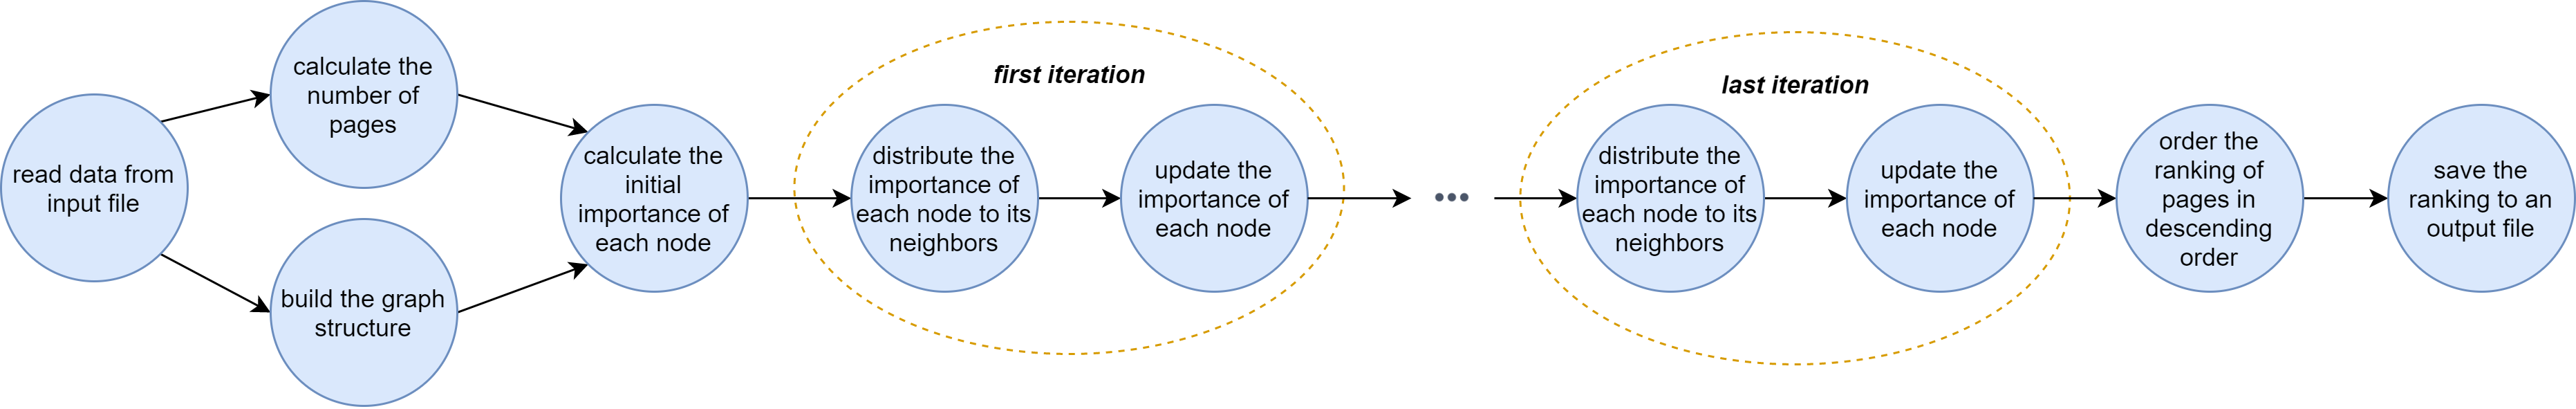
\includegraphics[width=\textwidth]{img/dag.png}
	\label{fig:parsingPhase}     
\end{figure}

\subsection{Performance Optimization}

\subsubsection{Partitioning}
Since Spark uses 2 worker nodes in order to execute the applications, and due to the independence of each input record from the others, the \textit{textFile} action is explicitly configured to use 2 parallel readers, so that to speed up this operation and not to exchange data across the network on the first partitioning (again we specify we want two partitions for the target RDD). Thanks to that and to the other optimizations reported in the following paragraphs, we can have \textbf{co-partitioned} join operations, which means no need for shuffling.


\subsubsection{Caching}
Once every worker has computed its own partition of the graph structure (nodes + outgoing links), it will be going to need this static data multiple times across the iterative computation. For this reason, workers are asked to \textbf{cache} in memory the \textbf{nodes} RDD (containing the graph structure), so that to avoid the recomputing of it across the iterations. This choice lead to a sensible performance boosting and required time reduction (more than 3 times less in a run with 5 iterations).

\noindent With small datasets, partitions of this RDD can fit completely in memory. On the contrary, huge datasets could degrade the performance gain, but in this case the disk persistency of the RDD is still a better choice rather than the full re-computation from scratch.   


\subsubsection{Shuffle Minimization}
Right after the flatMap operation applied to the joined RDD, we obtain a RDD of (page, contribution) records. Since we want to consider the initial pages only, we must consider the contributions destined to nodes inside the set of considered one. At this point we only have a (cached) nodes RDD and the contributions RDD, so we could:

\begin{itemize}
	\item Join the 2 RDDs through an inner join, which will automatically keep only the contributions that match a page included in the nodes RDD
	\item Take the keys of the \textit{nodes} (obtaining the keys list) and filter out contributions whose receiver is out of this \textit{keys} list
\end{itemize}

The first approach is obviously easier to develop but requires a \textbf{many-to-many} shuffling of a \textbf{very big data structure} (the contributions RDD); on the contrary with the second approach we can simply apply a filter to local data, keeping only records matching the predicate (belonging to the keys list): in this way we need \textbf{no data exchange} between workers. The main drawback is the fact that Spark does not allow to reference a RDD inside a transformation, thus we need to \textbf{explicitly collect} the keys RDD into a keys list.

\noindent The performance evaluation of the 2 alternative approaches shows a very significant improvement with the collect+filter strategy (till 2.5 times less) 

\subsubsection{Use of MapValues}
Every time is possible, the use of the mapValues is suggested since it does not modify the keys of the records, thus speeding up the computation and \textbf{preserving data partitioning}. In our case, we exploit this property twice:

\begin{enumerate}
	\item Once we have the \textit{nodes} RDD, made of (title, outgoingEdges) pairs, in order to compute the \textit{pageranks} RDD, it is pointless to re-read the titles from the input file and associate to each of them the initial value. A much faster approach is to take the \textit{nodes} RDD and remap the keys (titles) associating to them the initial value through a mapValues, so that to keep also the partitioning (every worker has a partition on nodes with the same pages that are in the corresponding partition of \textit{pageranks}. The collateral benefit is that the first join in the iteration \textbf{does not need an actual shuffling}.
	\item Right after the reduceByKey we obtain a list of (title, sum of contribution) pairs; from this data structure we need to compute the page ranks. Since this computation does not affect the key (does not depend on the title of the page), we simply use a mapValues   
\end{enumerate}

\subsection{Performance Evaluation}
To evaluate the performance of our algorithm, we considered three input files, with different numbers of pages. Precisely, we used the following files:

\begin{enumerate}
	\item \textbf{wiki-micro.txt}, which contains 2427 pages. This file is a pre-processed version of the Simple Wikipedia corpus in which the pages are stored in an XML format.
	\item \textbf{dataset5.txt}, which contains 5000 pages. This file is a synthetic dataset we created using the same structure as wiki-micro.txt. Each node has a random value of outgoing edges between 0 and 10.
	\item \textbf{dataset10.txt}, which contains 10000 pages. This file is a synthetic dataset we created using the same structure as wiki-micro.txt. Each node has a random value of outgoing edges between 0 and 10.
\end{enumerate}

In the graph below are the results obtained with 5, 10 and 15 iterations of the algorithm written in Java and the one written in Python for each of the three files.


\noindent As can be seen, the execution time grows fairly linearly with the number of iterations and the number of pages within the file. Also, we could not see a significant difference between the two implementations; we can actually say that they have essentially the same performance

\begin{figure}[H]
	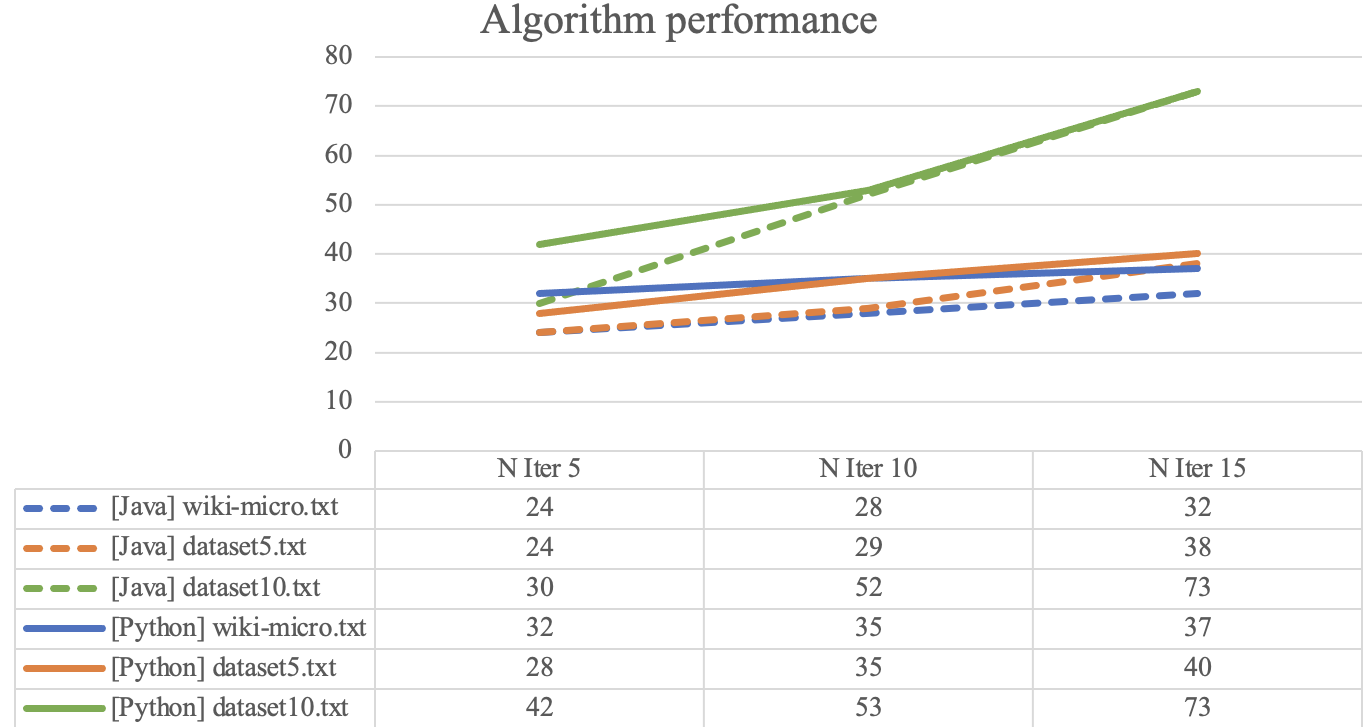
\includegraphics[width=\textwidth]{img/result.png}
	\label{fig:result}     
\end{figure}
